\chapter*{Preface}
This report is part of the fifth semester project made by project group SW510E16 at Aalborg University, Software Engineering starting from the 2nd of September to the 21st of December 2016. \newline
The project is based on the \textit{Aalborg-model} study method, where problem and project based learning is the focus. The theme of this semester is to make an embedded system with real-time constraints. The project group chose to make a trash bin that should be able to catch the trash thrown at it. \newline

Thank the people who should be thanked for helping making the project, here. 
\newline
\newline
\newline
\newline

{\Huge\textbf{Signatures}}
\newline
\newline

\begin{table}[H]
	\centering
		\begin{tabular}{c c c}
			\underline{\phantom{mmmmmmmmmmmmmm}} & \underline{\phantom{mmmmmmmmmmmmmm}} & \underline{\phantom{mmmmmmmmmmmmmm}} \\
			Christian Dannesboe			& Frederik Børsting Lund 		& Karrar Al-Sami 			\\
			&&\\
			&&\\
			\underline{\phantom{mmmmmmmmmmmmmm}} & \underline{\phantom{mmmmmmmmmmmmmm}} & \underline{\phantom{mmmmmmmmmmmmmm}} \\
			Mark Kloch Haurum			& Lasse Lyngø Nielsen 		& Søren Lyng 				\\
			&&\\
			&&\\
		 																		
		\end{tabular}
\end{table}

\chapter*{Reading guide}
Throughout the report sources are referred to by the Harvard citation method. When a source is listed in the report, the last name of the author and a publication year is listed. The sources are all listed alphabetically in  the \textit{\textbf{Bibliography}} section. \newline
\textit{This is an example of a source listed in the report: \textbf{\citep{safe}}.} \newline
The source may refer to either the whole section or to only that sentence. The way this differs depends on the placement of the dot. If the dot is after the source, then that source refers to the sentence and if the dot is before the source, then the source refers to the whole section. 


When referring to figures, tables and source code, numbers are used. Depending on which chapter and number of figure/table it is, the number is defined. \newline
\textit{This example can be used: In chapter X we want to refer to the second figure. This is done by giving the figure number \textbf{X.2}, where X is the number of the chapter we're referring from.}
\newline

When referring to source code, we're using code snippets. These code snippets aren't necessarily the full source code, but may be shorter version of it and/or missing comments. When code has been removed in the snippets, the use of three dots are used:  \textit\textbf{{"..."}}, these dots show that some code altering has been made in the snippet, whether it's because it's long and irrelevant for understanding the purpose of the code, or because we're simply just trying to explain those few lines. 

Throughout the report requirements are split into four colours with four different meanings. The colour blue refers to new requirements or focus requirements for that specific increment. The colour green refers to a requirement being fulfilled. Orange means that the requirement is fulfilled but has been changed. Red means that the requirement has been changed, but not yet fulfilled. 


\chapter*{Process model}
\label{Process model}
The process model is a meld of elements from both plan driven and agile development. The process is plan driven in so far as to include a clear goal of what the initial requirements of the system are. The process model is very agile in that, although there is a clear outline as to what the requirements are, these are incrementally approached, with a simple starting point becoming increasingly covering of the project vision through the subsequent increments. The reason the group approached this project with our 'own' process model is to better explain what we're actually doing, rather than forcing ourselves into picking a development method and try to explain what we're doing according to that method.

The increments will be split up into four sections. Initially some of the already known requirements will be considered from previous increments and for the first increment from the analysis and hardware chapters, and these requirements will be the topic of the increment.
After the initial requirement consideration, a design phase follows which details the design and problem considerations preceding the implementation. The design phase is then followed by an implementation phase which will explain the implementation process. The final phase is an evaluation of the increment and will concern whether the requirements were fulfilled, if an requirement needs to be altered, or if an requirement will be continued in the following increment. The evaluation will also include several tests of the implementation, in order to see what works and what doesn't work. The evaluated requirements from an increment will then become the starting point of the next increment. 

The process includes emphasis on a small group of individuals with tasks usually undertaken by two group members or more, which is to promote cooperation and attempt to avoid having a single individual involved in a task beyond their capabilities and to get a second opinion. This is also to ensure that information is quickly communicated and exchanged by group members. The process uses pair programming because it promotes better programming and is usually very motivating in socially engaging issues with cooperation of project members.

\begin{figure}[h]
\centering
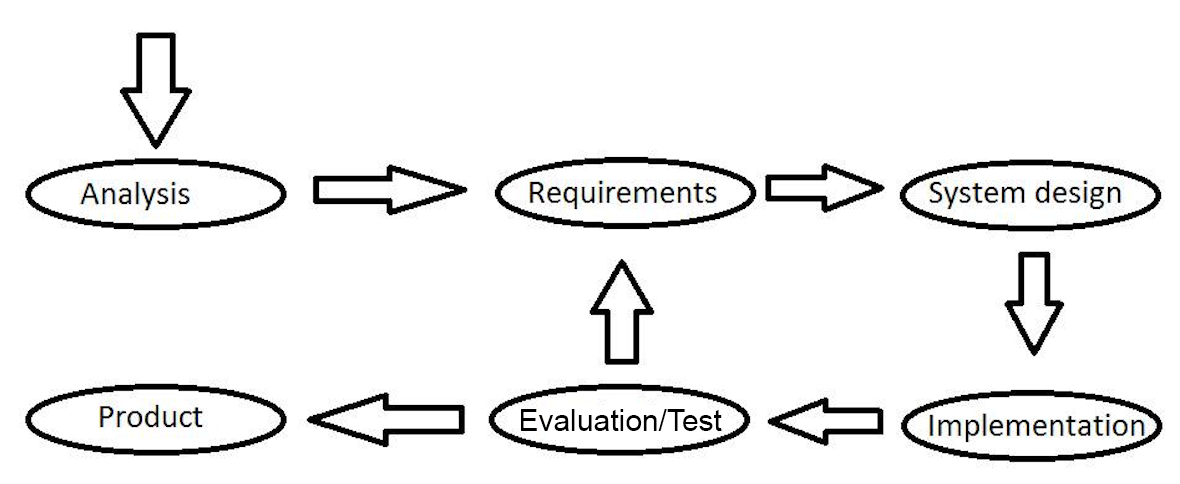
\includegraphics[scale=0.30]{billeder/process-model}
\caption{Process model used for the project}
\label{pm}
\end{figure}

\chapter*{Toolchain}
The following tools has been used to create the report and the product of the project. Every tool in the toolchain has a description stating the benefits and use of the tool.

\begin{itemize}
	\item GitHub
	\item TeX Studio
	\item Visual Studio C\#
	\item Arduino IDE 1.0.3
	\item BoundT
	\item UPPAAL
\end{itemize}

\section*{Use of tools}
\textbf{GitHub} is used with the intention of merging and sharing documents. This tool is also used here to verify each version of the documentation and code, to ensure that everyone has the latest update of the project.\newline
\textbf{TeX Studio} is used as a writing environment when writing with the markup language LaTeX. After some experience it has proven to be a great tool for creating a report. This tool in concoction with GitHub makes it possible to work on the project in pairs or alone, with little merging conflicts. \newline
\textbf{Visual Studio C\#} is used in this project to create the C\# code for the Kinect. \newline
\textbf{Arduino IDE 1.0.3} is used in this project to code the Arduino. Any later IDE is not suitable for this project, which will be explained in the report. \newline
\textbf{BoundT} is used to calculate the bounds of the code, which will be used in a WCET-analysis. \citep{boundt} \newline
\textbf{UPPAAL} is an integrated tool environment for modeling, validation and verification of real-time system. \citep{uppaal}